\documentclass[12pt]{article}
\usepackage{amssymb,amsmath,mathrsfs,color}
\usepackage[utf8]{inputenc}
\usepackage[T2A]{fontenc}
%\usepackage[frenchb]{babel}
\usepackage[russian,english]{babel}
%\usepackage{aeguill}
\usepackage{graphicx}
\usepackage{mathrsfs}
%
%\textheight = 22cm
%\textwidth = 15cm
%\hoffset = -1,4cm
%\voffset = - 3cm
%\parskip = 0.5mm
\def\hbr{\hfil\break}
%\newcommand\F{\mbox{I\kern-2pt F}}
%%\newcommand\r{\rightarrow}
%\newcommand\cA{{\cal A}}
%\newcommand\cE{{\cal E}}
%\newcommand\cF{{\cal F}}
%\newcommand\cG{{\cal G}}
%\newcommand\cL{{\cal L}}
%\newcommand\cB{{\cal B}}
%\newcommand\cN{{\cal N}}
%\newcommand\cX{{\cal X}}
%\newcommand\cM{{\cal M}}
%\newcommand\cH{{\cal H}}
%\newcommand\cP{{\cal P}}
%\newcommand\cC{{\cal C}}
%\newcommand\e{\varepsilon }
%\newcommand\fdem{{$\Box$}}
\newcommand\dm{{\sl Доказательство. }}
\newtheorem{theo}{Теорема}[section]
\newtheorem{prop}[theo]{Предложение}
\newtheorem{lemm}[theo]{Лемма}
\newtheorem{coro}[theo]{Следствие}





%\documentclass[ 12pt,article]{amsart}
%\documentclass[12pt, letterpaper]{amsart}
\usepackage{graphicx, amssymb, color}
\usepackage{hyperref}
%\usepackage{refcheck}

\addtolength{\hoffset}{-1.9cm}
\addtolength{\textwidth}{3.8cm}
\addtolength{\voffset}{-0.7cm}
\addtolength{\textheight}{1.4cm}


\renewcommand{\baselinestretch}{1.31}




\newcommand\cA{{\mathcal A}}
\newcommand\cE{{\mathcal E}}
\newcommand\cC{{\mathcal C}}
\newcommand\cF{{\mathcal F}}
\newcommand\cG{{\mathcal G}}
\newcommand\cI{{\mathcal I}}
\newcommand\cK{{\mathcal K}}
\newcommand\cL{{\mathcal L}}
\newcommand\cB{{\mathcal B}}
\newcommand\cN{{\mathcal N}}
\newcommand\cM{{\mathcal M}}
\newcommand\cX{{\mathcal X}}
\newcommand\cD{{\mathcal D}}
\newcommand\cO{{\mathcal O}}
\newcommand\cR{{\mathcal R}}
\newcommand\cP{{\mathcal P}}
\newcommand\cQ{{\mathcal Q}}
\newcommand\cS{{\mathcal S}}
\newcommand\cT{{\mathcal T}}
\newcommand\cU{{\mathcal U}}
\newcommand\cV{{\mathcal V}}
\newcommand\cY{{\mathcal Y}}
\newcommand\cZ{{\mathcal Z}}
\newcommand\cW{{\mathcal W}}

\newcommand\bF{{\bf F}}
\newcommand\bP{{\bf P}}
\newcommand\bQ{{\bf Q}}
\newcommand\bT{{\bf T}}
\newcommand\fP{{\mathfrak P}}

%\newcommand\E{{\mathbb E}}
%\newcommand\T{{\mathbb T}}
%\newcommand\Y{{\mathbb Y}}
%\newcommand\R{{\mathbb R}}
%\newcommand\N{{\mathbb N}}
%\documentclass[12pt, letterpaper]{amsart}
\usepackage{graphicx, amssymb, color}
\usepackage{hyperref}
%\usepackage{refcheck}

\newcommand\D{{\mathbb D}}
\newcommand\E{{\mathbb E}}
\newcommand\T{{\mathbb T}}
\newcommand\Y{{\mathbb Y}}
\newcommand\R{{\mathbb R}}
\newcommand\N{{\mathbb N}}
\newcommand\e{{\varepsilon}}
%\newcommand\dm{{\sl Доказательство}}
%\newtheorem{theo}{Theorem}[section]
%\newtheorem{prop}[theo]{Proposition}
%\newtheorem{lemm}[theo]{Lemma}
%\newtheorem{coro}[theo]{Corollary}
%\newtheorem{defin}[theo]{Definition}
%%\newtheorem{rem}[theorem]{Remark}
%\newtheorem{rem}[theo]{Remark}

\newcommand\fdem{$\Box$}
\newcommand\beq{\begin{equation}}
\newcommand\eeq{\end{equation}}
\newcommand\bea{\begin{eqnarray}}
\newcommand\eea{\end{eqnarray}}
\newcommand\bean{\begin{eqnarray*}}
\newcommand\eean{\end{eqnarray*}}

%\renewcommand{\theequation}{\thesection.\arabic{equation}}
%\renewcommand{\thetheo}{\thesection.\arabic{theo}}
%\renewcommand{\theprop}{\thesection.\arabic{prop}}
%\renewcommand{\thelemm}{\thesection.\arabic{lemm}}
%\renewcommand{\therem}{\thesection.\arabic{rem}}
%\renewcommand{\thedefin}{\thesection.\arabic{def}}
\begin{document}
\centerline{\bf \Large ЭКЗАМЕН 2021}
%Exam 2020 (2nd year students)}
\bigskip 
%\centerline{\bf Фамилия И.О. }
%\centerline{\bf Name}
%\centerline{\bf Test 1}
\bigskip
\bigskip
Во всех  задачах $w$ --- винеровский процесс, $\Lambda_t=t$.  

\medskip
\noindent
{\bf 1.} 
Покажите, что процесс  $B_t=w_1-w_{1-t}$ --- винеровский на отрезке $[0,1]$. 


\medskip
\noindent
{\bf 2.} 
Выпишите  решение СДУ $dX_t=-(1/2)X_tdt +w_t$, $X_0=0$,  и покажите, что $X_{\ln (t+1)}\sqrt {t+1} $ --- винеровский процесс.  
Пользуясь законом повторного логарифма вычислите $\limsup_{t\to \infty} X_t/\sqrt t$.  


\medskip
\noindent
{\bf 3.} 
Докажите, что $w$ --- мартингал относительно фильтрации $(\cF^o_{t+})$, где $\cF^o_t:=\sigma\{w_s,\ s\le t\}$. 

\medskip
\noindent
{\bf 4.} 
Пусть $(w,\cF)$ --- измеримое пространство с  фильтрациeй ${\bf F}=(\cF_t)_{t\ge 0}$.   На множестве 
$w\times \R_+$  определены  $\sigma$-алгебры $\cP:=\sigma\{ A\times ]s,\infty[, \  A\in \cF_s,\ s\ge 0, \ B\times \{0\},\  B\in\cF_0\}$   (предсказуемая) и $\cO:=\sigma\{A\times [s,\infty[, \ A\in \cF_s, \  s\ge 0\}$ (опциональнaя). Какая из них включает другую? 

\medskip
\noindent
{\bf 5.}  Пусть   $M^n\in \cM^{2,c}_0$,  $\langle M^n\rangle\le C={\rm const} $  и $\langle M^n\rangle_t\to t$        при  $n\to \infty$. Показать, что распределения случайных величин  $M^n_t$ слабо сходятся к гауссовскому  распределению с нулевым средним и дисперсией $t$. 

\medskip
\noindent
{\bf 6.}  Пусть $X^x$ --- решение  СДУ $dX^x_t=f(X^x_t)dt +g(X^x_t)dw_t$, $X^x_0=x$,  где $f,g\in C^1$, $f'$ и $g'$ ограничены, и пусть $Y$  --- решение СДУ $dY_t=f'(X^x_t)Y_tdt +g(X^x_t)Y_tdw_t$, $Y_0=1$. Показать, что  $Y_t$ --- производная функции  $x\mapsto X_t^x$.

\medskip
\noindent
{\bf 7.}  По теореме о предсказуемом  представлении $w_1^4=E w_1^4+\varphi\cdot w_1$, где $\varphi\in L^{2,2}$. Найти $\varphi$. 

\medskip
\noindent
{\bf 8.}  
Пусть динамика управляемoгo процессa зaдаётся СДУ
$dX_t=(u_t-\rho X_t)dt +\sigma X_tdw_t$, 
где управление $(u_t)_{t\le T}$ --- предсказуемый процесс со значениями в  $[0,M]$. Цель: при заданном начальном условии максимизировать 
$$
\E \Big(\gamma X_T- \int_0^T e^{-ct}u_t dt\Big).
$$
Записать уравнение Беллмана.  
 

\medskip
\noindent
{\bf 9.} Цена рискового актива  $S=x+a\Lambda +\sigma w$. Процентная ставка равна нулю. Получить формулу для цены опциона колл. 

\medskip
\noindent
{\bf 10.} Определить цену опциона колл  с погашением через 180 дней по модели BS.  Цена
акции 95, страйк 105, волатильность 11, процентная ставка  2. 

\section{Решения}
\subsection{Задача 1}
Отметим, что процесс $B$ согласован с фильтрацией $\cG_t = \sigma(w_1-w_{1-s} : s \leq t)$. Также для $0\leqs < t \leq 1$ выполнено
\[B_t-B_s = w_{1-s}-w_{1-t} \]
и так как винеровский процесс $w$ имеет независимые приращения, нетрудно проверить, что $B_t-B_s$ независим с $\cG_s$. Очевидно, что $B_t-B_s$ имеет Гауссово распределение $\cN(0, t-s)$ и $B_0 = 0$, значит, по определению заключаем, что $B$ есть винеровский процесс.
\subsection{Задача 2}
Ищем такую замену, чтобы в правой части $X_t$ не было и мы смогли проинтегрировать.\\
a) Пусть $Y_t=f(x,t)=x e^{\frac{t}{2}},$ следовательно $f'_t=\frac{1}{2}e^{\frac{t}{2}}x, \quad f'_x=e^{\frac{t}{2}},\quad f''_{xx}=0.$\\
Получаем
$$dY_t=f'_tdt+f'_xdX_t+\frac{1}{2}f''_{xx}(dX_t)^2$$
$$dY_t=(\frac{1}{2}e^{\frac{t}{2}}X_t)dt + e^{\frac{t}{2}}(-\frac{1}{2}X_tdt+dw_t)$$
$$dY_t=(\frac{1}{2}e^{\frac{t}{2}}X_t-\frac{1}{2}e^{\frac{t}{2}}X_t)dt+e^{\frac{t}{2}}dw_t=e^{\frac{t}{2}}dw_t$$
Получили, что $d(e^{\frac{t}{2}}X_t)=e^{\frac{t}{2}}dw_t$, следовательно $e^{\frac{t}{2}}X_t-e^0X_0=\int\limits_0^te^{\frac{s}{2}} dw_s$\\
Ответ: $X_t=\int\limits_0^te^{\frac{s-t}{2}} dw_s$\\
b.1) Первый способ:\\
$Z_t=X_{\ln{(t+1)}}\sqrt{t+1}\Rightarrow Z_t=\sqrt{t+1}X_{\ln{(t+1)}}=\sqrt{t+1}e^{-\ln{\frac{(t+1)}{2}}}\int\limits_0^{ln{(t+1)}}e^{s/2}d w_s = \int\limits_0^{ln{(1+t)}}e^\frac{u}{2}dw_u=f\cdot w_{ln(1+t)},$ где $f=e^{\frac{u}{2}}.$\\
Посчитаем $<Z_t>=\int\limits_0^{ln{(t+1)}}e^udu=t\Rightarrow$ по теореме Леви $Z_t$ — винеровский процесс.\\

b.2) Второй способ:\\
Покажем, что $Z_t=X_{\ln(t+1)}\sqrt{t+1}$ винеровский процесс.\\

Мы уже знаем, что\\
$X_t=e^{-\frac{t}{2}}\int_{0}^{t}e^{\frac{s}{2}}dw_s$\\

Значит\\
$Z_t=\sqrt{t+1}X_{ln(t+1)}=\sqrt{t+1}e^{-\frac{\ln(t+1)}{2}}\int_{0}^{\ln(t+1)}e^{\frac{s}{2}}dw_s=\int_{0}^{\ln(t+1)}e^{\frac{u}{2}}dw_u$\\

Пусть $s<t$\\
Тогда $Z_t-Z_s$ Гауссовский процесс, ведь $Z_t$ Гауссовский как предел гауссовских величин.\\

Итак:\\
$E(Z_t-Z_s)=0$\\

Далее по свойству изометрии Ито:\\

$E(Z_t-Z_s)^2=\int_{\ln(s+1)}^{\ln(t+1)}e^{u}du=t-s$\\

Значит\\

$Law(Z_t-Z_s)= N(0,t-s)$\\

Итак, $Z_t$ винеровский процесс.


c) Найти $\lim\sup_{t\to\infty} \frac{X_t}{\sqrt{t}}$\\
Имеем: $\lim\sup_{t \to \infty}\frac{w_t}{\sqrt{2t\ln\ln t}}=1$ верно п.н. в силу закона повторного логарифма. \\
$$w_t=X_{\ln{(t+1)}}\sqrt{t+1}\Rightarrow w_{e^t-1}=X_{\ln{e^t}}\sqrt{e^t}=X_te^{\frac{t}{2}}\Rightarrow X_t=\frac{w_{e^t-1}}{e^{\frac{t}{2}}}$$\\
Получается, что нужно найти:
$\lim\sup_{t\to\infty}\frac{w_{e^t-1}}{\sqrt{t}e^{\frac{t}{2}}}$.
Сделаем замену $s=e^t-1\Rightarrow t=\ln(s+1).$\\
Получаем
$$\lim\sup_{t\to\infty}\frac{w_{e^t-1}}{\sqrt{t}e^{\frac{t}{2}}}=\lim\sup_{s\to\infty}\frac{w_s}{\sqrt{s+1}\sqrt{\ln(s+1)}}=\lim\sup_{s\to\infty}\frac{w_s}{\sqrt{2s\ln\ln s}}\sqrt{\frac{2s\ln\ln s}{(s+1)\ln(s+1)}}\to 0$$
Так как $\lim\sup_{s\to\infty}\frac{w_s}{\sqrt{2s\ln\ln s}} \to 1$, а $\frac{2s\ln\ln s}{(s+1)\ln(s+1)} \to 0$ п.н.\\
Ответ: $\lim\sup_{t\to\infty}\frac{X_t}{\sqrt{t}}= 0$

\subsection{Задача 3}
$\cF^o_{t+} = \cap_{m \in \mathbb{N}}\cF^o_{t+\frac{1}{m}}$, где $\cF^o_t:=\sigma\{w_s,\ s\le t\}$.
\[E(w_t | \cF_{s+}) = E(w_t | \cap_{m \in \mathbb{N}}\cF^o_{s+\frac{1}{m}}) = E(w_t | \cF_s^o) = E(w_t-w_s | \cF_s^o) + E(w_s | \cF_s^o) = E(w_t-w_s) + w_s = w_s\]
Здесь мы воспользовались непрерывностью $\sigma$-алгебры и независимостью $w_t-w_s$ от $\cF_s^o$.\\
Вышеприведенные выкладки приводят к заключению, что винеровский процесс действительно является мартингалом относительно указанной фильтрации.

\subsection{Задача 4}
Рассмотрим несколько случаев: $s>0$ и $s=0$.
Если $s>0$, то понятно, что 
\[\{A\times ]s,\infty[, \ A\in \cF_s, s\ge 0\}\subseteq\{A\times [s,\infty[, \ A\in \cF_s, s\ge 0\}\] и всегда $\{B\times \{0\},\ B\in\cF_0\}\subseteq\cO.$
Если $s=0$, то $\{A\times ]0,\infty[, \ A\in \cF_0,\ B\times \{0\},\ B\in\cF_0\}=\{ B\times ]0,\infty[, \ B\times \{0\},\ B\in\cF_0\}=\{A\times [0,\infty[, \ A\in \cF_0\}\subseteq\cO.$
Таким образом, выполнено включение
$\cP \subseteq\cO $.

\subsection{Задача 5}
Имеем:
\[
e^{i \lambda M_t^n}=1+i \lambda \int\limits_0^t e^{i \lambda M_s^n} \, dM_s^n - \frac12 \lambda^2 \int\limits_0^t e^{i \lambda M_s^n} \, d <M_s^n>
\]
\[
\phi _t^n=1-\frac12 \lambda^2 \textbf {E} \int\limits_0^t e^{i \lambda M_s^n} \, d <M_s^n>
\]
\[\phi_0^n=1\]
По определению стохастического интеграла
\[\int_0^t e^{i \lambda M_s^n} d<M_s^n> = \lim_{max_i |t_{i+1} - t_i| \to 0} \sum_{j=0}^k e^{i \lambda M_{t_j}^n} (<M_{min(t_{j + 1}, t)}^n> - <M_{min(t_{j}, t)}^n>) \]

где $0 = t_0 < t_1 < \ldots <  t_{k+1} = T$.

Перейдем к пределу $n \to \infty $ : 
Тогда 
\[\lim_{n \to \infty}\int_0^t e^{i \lambda M_s^n} d<M_s^n> =\lim_{n \to \infty} \lim_{max_i |t_{i+1} - t_i| \to 0} \sum_{j=0}^k e^{i \lambda M_{t_j}^n} (<M_{min(t_{j + 1}, t)}^n> - <M_{min(t_{j}, t)}^n>) \]
Так как $ <M_s^n>\leqslant C$ и сумма конечная, то внутренний предел существует, значит имеем право поменять пределы местами.
\[\lim_{n \to \infty}\int_0^t e^{i \lambda M_s^n} d<M_s^n> = \lim_{max_i |t_{i+1} - t_i| \to 0} \lim_{n \to \infty} \sum_{j=0}^k e^{i \lambda M_{t_j}^n} (<M_{min(t_{j + 1}, t)}^n> - <M_{min(t_{j}, t)}^n>) = \]
\[= \lim_{max_i |t_{i+1} - t_i| \to 0} \sum_{j=0}^k e^{i \lambda t_j} (min(t_{j + 1}, t) - min(t_{j}, t)) \]

Возьмем матожидание от обеих частей по теореме Фубини, тогда:
\[ \phi_t=1-\frac12 \lambda^2 \int\limits_0^t \phi_s \,ds \]
Это верно, так как $<M_s^n> \to s $ и $ <M_s^n>\leqslant C$
\[\phi_0=1\]
Следовательно $ \phi_t=e^{-\frac12 \lambda^2 t} $, то есть получили характеристическую функцию Гауссовского распределения с нулевым
средним и дисперсией t.
\subsection{Задача 6}
Остается для следующих поколений.
\subsection{Задача 7}
По теореме о предсказуемом представлении $\xi = E\xi + \phi w_T$. Также известно, что $Ew_1^4 = 3$, значит
\[w_1^4 = 3 + \int _0^1 \phi_t d w_t\]
\[X_t = E(X_t | \cF_t) = E(w_1^4 |\cF_t ) = E((w_1 - w_t + w_t)^4 |\cF_t ) = \]
\[ =E((w_1 - w_t)^4 + 4(w_1 - w_t)^3 w_t + 6(w_1 - w_t)^2 w_t^2 + 4(w_1 - w_t)w_t^3 + w_t^4 | \cF_t) = \]
\[= 3(1-t)^2 + 6w_t^2 (1-t) + w_t^4\]
Имеем: $X_t=3(1-t)^2+6w_t^2(1-t)+w_t^4$.
\newline
Положим $f(x,t):=3(1-t)^2+6x^2(1-t)+x^4$, значит, $f'_t=-6(1-t)-6x^2$, $f'_x=12x(1-t)+4x^3$, $f''_{xx}=12(1-t)+12x^2$.
\newline
По формуле Ито для функции $f$ имеем:
\begin{equation*}
\begin{split}
&dX_t=(-6(1-t)-6w_t^2)dt+(12w_t(1-t)+4w_t^3)dw_t+\frac 12(12(1-t)+12w_t^2)dt=\\
&=(-6(1-t)-6w_t^2+6((1-t)+w_t^2))dt+(12w_t(1-t)+4w_t^3)dw_t
\end{split}
\end{equation*}
Значит, $\phi_t=12w_t(1-t)+4w_t^3$, а $\phi_1=4w_1^3$.

\subsection{Задача 8}
Данное СДУ $dX_t=(\mu_t-\rho X_t)dt+\sigma X_tdw_t$, а мы хотим:
$$E(\gamma X_T -\int_0^T e^{-ct}u_tdt)\to max.$$
Пусть $W(t,X)=\sup_{X_t=x, \pi\in A(x,t)} E(\gamma X_T -\int_t^T e^{-cs}u_s ds)$. Пусть $f\in C^{1,2} ([0,T]\times\mathbb{R_+})$ и\\ $f(T,x)=\gamma x$. Рассмотрим $Y_t=f(t, X_t)-\int_0^t e^{-cs}u_s ds$ и $X_0=x$.

Если для всех стратегий это супермартингал, то
$$EY_T=E(\gamma X_T-\int_0^T e^{-ct}u_t dt)\le f(0,x)=EY_0$$
Если для какой-то стратегии это мартингал, то для неё
$$E(\gamma X_T-\int_0^T e^{-ct}u_t dt)=f(0,x) \Rightarrow W(0,x)=f(0,x)$$
По формуле Ито:
$$dY_t=\underbrace{\left( \frac{\partial f}{\partial t}+\frac 12 \frac{\partial^2 f}{\partial x^2} \sigma^2 X_t^2 +\frac{\partial f}{\partial x}(u_t-\rho X_t) -e^{-ct} u_t\right)}_{=:L^{u_t}f(t,X_t)}dt +\frac{\partial f}{\partial x}\sigma X_tdw_t$$
В итоге, уравнение Беллмана имеет вид:
$$\sup_u\left(\frac{\partial f}{\partial t}+\frac 12 \frac{\partial^2 f}{\partial x^2} \sigma^2 x^2 +\frac{\partial f}{\partial x}(u-\rho x) -e^{-ct} u\right)=0$$
\subsection{Задача 9}
$\xi=p+H\cdot S_t$\\
$H\cdot S_t=H(a\cdot\Lambda_T+\sigma\cdot w_T)=Ha\cdot\Lambda_T+H\sigma\cdot w_T$\\
$\tilde {w_t}:= w_t+\frac{a}{\sigma}\cdot\Lambda_t\Rightarrow \phi_t=H_t\cdot\sigma\Rightarrow\xi=p+\phi\cdot \tilde w_T\Rightarrow \tilde W$ — винеровский по теореме Гирсанова $\Rightarrow$ по теореме о предсказуемом представлении $p =\tilde E\xi$, по мере $\tilde P = P e^{\frac{-a}{\sigma}\cdot W-\frac{1}{2}\frac{a^2}{\sigma^2}\cdot\Lambda}.$\\
Свели задачу к случаю, когда $$dS_t=S_t(adt+\sigma dw_t)$$
Далее получаем цену опциона в момент $t$
$$C(t,x,\sigma)=x\Phi(d)-K\Phi(d-\sigma\sqrt{T-t}),$$
$d=d(t,x,\sigma)=\frac{1}{\sigma\sqrt{T-t}}\ln{\frac{x}{K}}+\frac{1}{2}\sigma\sqrt{T-t}$.
\subsection{Задача 10}
Решение: Для того, чтобы определить цену опциона ``колл'' с дисконтированным платежом воспользуемся формулой
$$C(0,T,\sigma)=x\Phi(d_1(0,x))-Ke^{-rT}\Phi(d_2((0,x)), \text{ где }$$
$$d_1(0,x)=\frac{1}{\sigma \sqrt T}\ln\frac xK +\frac 12 \sigma\sqrt T+\frac r\sigma \sqrt T, \; d_2(0,x)=d_1(0,x)-\sigma\sqrt T$$
Вычислим сначала $d_1$ и $d_2$:
$$d_1(0,x)=\frac{1}{0,11 \sqrt {\frac{180}{365}}}\ln\frac{95}{105} +\frac{1}{2} 0,11\sqrt\frac{180}{365}+\frac {0,02}{0,11} \sqrt\frac{180}{365}\approx -1,295626431+0,16630483\approx-1,129321601$$
$$d_2(0,x)=-1,129321601-0,11\sqrt\frac{180}{365}\approx-1,206568759$$
Следовательно,
$$C(0,\frac{180}{365},0,11)=95\Phi(-1,129321601)-105e^{-\frac{360}{365}}\Phi(-1,206568759)\approx 0,459568194$$
Также приведем программный код, подтверждающий наши выкладки

\begin{figure}[h]
\centering
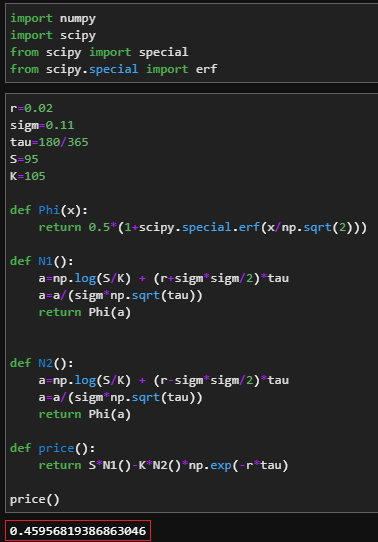
\includegraphics[scale=1]{images/1.png}
\caption{Численные выкладки в 10 задаче.}
\end{figure}



\end{document}